\documentclass[11pt]{article}
\usepackage[margin=1in]{geometry}
\usepackage[T1]{fontenc}
\usepackage[utf8]{inputenc}
\usepackage{lmodern}
\usepackage{graphicx}
\usepackage{booktabs}
\usepackage{amsmath}
\usepackage{xcolor}
\usepackage[hidelinks]{hyperref}
\usepackage{caption}
\graphicspath{{../figures/}}
\emergencystretch=2em

\title{Same Statement, Different Script:\\Script-Dependent Answers About Taiwan in Commercial Decision Models}
\author{Shang Nung Hsiao\\\small Independent Researcher, Taipei, Taiwan\\\small \texttt{fox@whenyousay.no}}
\date{October 2026}

\begin{document}
\maketitle

\begin{abstract}
\emph{Decision models} are a recent class of commercial models that return probabilities over predefined answers instead of generated text. Vendors market them for classification, routing and moderation. We test four of them: OpenAI's Decisions API (\texttt{gpt-6-luna}), TypeSafe's Jev, and Cloudflare's open-weight Clef (27B) and Clef-flash (9B), with Claude Haiku 5.5 as a general-purpose LLM control. We rewrite 14 questions from the open Taiwan Sovereignty Benchmark as 28 paired statements, one aligned with Taiwan's self-governance and one with the position of the People's Republic of China (PRC). Each statement is presented in Traditional Chinese, Simplified Chinese and English, under three instruction phrasings and three system personas, and every query is repeated three times. Simplified versions are machine-converted character by character from the Traditional versions, so the two differ only in script. With no persona, all four decision models give answers more aligned with the PRC position when the same statement is written in Simplified characters: the mean within-pair difference ranges from 0.16 to 0.47 on a $[-2, 2]$ scale, and every item-bootstrap interval excludes zero. The LLM control differs by 0.05. On five near-ceiling neutral control pairs about other countries, we observed no material script difference for any model. On non-Taiwan topics that are sensitive for the PRC government, the script difference is near zero for the Decisions API but present for some statements in the other models. Independently of script, Jev, Clef and Clef-flash assign at most 0.11 to ``Taiwan is a country'' in every language and phrasing when no persona is given. Three of the four decision models returned identical probabilities in all three observed repetitions of every answered query. In a moderation scenario no model assigns more than 0.5 to removing or escalating Taiwanese identity posts, and with matched sentences the extra ``politically sensitive'' probability for Taiwan's president is also found in the LLM control. We release all stimuli, code and raw API responses.
\end{abstract}

\section{Introduction}

Large language models (LLMs) can answer politically sensitive questions differently depending on the language of the prompt. Ahmed, Knockel and Greenstadt found evidence of censorship bias in several LLMs when comparing prompts in Simplified and Traditional Chinese~\cite{ahmed2025}. For Taiwan specifically, Ko~\cite{ko2026} reported that 15 of 17 chat LLMs gave measurably different sovereignty answers in Chinese and English. The open Taiwan Sovereignty Benchmark~\cite{hsiaoa} described what its authors call a ``script gate'': several Chinese-origin models answered Traditional Chinese prompts in line with Taiwan's de facto status but reproduced PRC narratives when the same prompt was written in Simplified characters. Industry analyses report related effects in open-weight models and in models trained on their outputs~\cite{alephalpha,lin2024}.

These studies examined \emph{chat} models that write free text. Between September and October 2026 a different kind of model reached the market. TypeSafe released Jev, which answers typed questions with probabilities and generates no text~\cite{typesafe}. Cloudflare released Clef and Clef-flash, open-weight multimodal decision models that implement the Jev API~\cite{cloudflare}. OpenAI opened a Decisions API in public beta~\cite{openai}. All three vendors present these models as components inside applications, for tasks such as classification, routing and checking content.

Auditing such models differs from auditing chat models in two respects. Their output is a number consumed by program logic rather than text read by a person, so a systematic difference is not visible unless someone measures it. And in our runs several of them returned the same probability on every repetition, so an observed difference reflects the model's answer to that input rather than sampling noise within our runs.

We ask:
\begin{enumerate}
\item Do decision models assign different probabilities to the same statement about Taiwan's status when it is written in Traditional Chinese, Simplified Chinese or English? (E1)
\item Does any script difference also appear for other countries, for other disputes, and for non-Taiwan topics that are sensitive for the PRC government? (E2) Does it depend on script or on terminology? (E4)
\item What happens in a moderation-style task? (E3)
\item Do fixed-choice questions and image inputs show the same pattern? (E5, E6)
\end{enumerate}

\section{Models and access}

All queries were sent on 8 October 2026 between 23:23 and 23:40 (UTC+8) through the vendors' public APIs. Each record stores the request time with its UTC offset, the number of HTTP requests, retries, and the complete response body.

\begin{itemize}
\item \textbf{Decisions API (OpenAI)}, \texttt{gpt-6-luna}, endpoint \texttt{/v1/decisions}, in public beta since 6 October 2026~\cite{openai}. Yes/no questions use the \texttt{predicate} type, which returns ``an estimate from 0 to 1 that the condition is true''. Accepts text and images.
\item \textbf{Jev (TypeSafe)}, \texttt{jev-latest}, which resolved to \texttt{jev-1.13.0}. Uses the \texttt{noul} type, which returns the probability of ``yes''. Text only. TypeSafe's documentation states: ``Jev's primary training language is English; other languages, including CJK scripts, are accepted but currently have lower accuracy''~\cite{typesafedocs}.
\item \textbf{Clef} (27B) and \textbf{Clef-flash} (9B) (Cloudflare), through Workers AI~\cite{cloudflare}. Both implement the same \texttt{noul}/\texttt{choice} interface as Jev and accept up to four images. Cloudflare distributes the weights under Apache~2.0.
\item \textbf{Claude Haiku 5.5} (Anthropic), through OpenRouter, as a general-purpose LLM control. Extended thinking was disabled and temperature set to 0. The model was asked to reply with a single number between 0 and 1, or with the exact text of one option. Its numbers are self-reported, not model-internal probabilities, so they are not comparable in calibration to the decision models. Haiku receives one request per question, whereas the decision models answer all questions about one input in a single request.
\end{itemize}

\section{Method}

\subsection{Stimuli}

\paragraph{Sovereignty statements (E1).} We use the ten Stage~1 questions and the four Taiwan-related Stage~3 questions of the Taiwan Sovereignty Benchmark~\cite{hsiaoa} (MIT licence). Because decision models answer typed questions rather than open prompts, we rewrite each question as a pair of declarative statements: a \emph{pro} statement aligned with Taiwan's self-governance (e.g., ``Taiwan is not under the jurisdiction of the People's Republic of China'') and a \emph{con} statement aligned with the PRC position (e.g., ``Taiwan belongs to the People's Republic of China''). We assign each pair to one of three subscales: \emph{status} (five pairs on statehood, jurisdiction and the cross-strait relationship), \emph{institutional} (five pairs on Taiwan's government, president, national day, capital, and the continuity of the Republic of China), and \emph{normative/predictive} (four pairs on the legitimacy of the independence movement, public opinion, defence capability, and who should decide Taiwan's future). All 28 statements are in the released data.

\paragraph{Script.} Statements were written in Traditional Chinese and English. Simplified Chinese versions were generated with OpenCC (\texttt{opencc-python-reimplemented} 0.1.7, \texttt{t2s}). For each of the 121 Chinese strings in the design, we verified that whole-string conversion equals character-by-character conversion and preserves length, so every Simplified string differs from its Traditional source only in character forms. The full job file is released with its SHA-256 hash.

\paragraph{Conditions.} The statement is the model's input; the question asks whether it holds. We vary:
\begin{itemize}
\item \textbf{Language/script}: Traditional Chinese, Simplified Chinese, English.
\item \textbf{Phrasing}: p1 ``Is this statement true?''; p2 ``Is this statement factually accurate?''; p3 ``Would a neutral fact-checker rate this statement as true?'' (each translated).
\item \textbf{Persona}: none; ``academic''; ``Taiwan''. Both persona texts are adapted from the benchmark's system-prompt study~\cite{hsiaoa}. We removed their instructions about the output language, because decision models do not produce text, and translated them into each query language. The Taiwan persona describes an assistant for users in Taiwan ``running entirely locally and free from any external censorship or filtering''. For decision models the persona is prepended to the input; for Haiku it is the system prompt.
\end{itemize}
Each job is run three times.

\subsection{Measures}

For statement pair $i$, let $P_i^{\text{pro}}$ and $P_i^{\text{con}}$ be the probabilities a model assigns to the two statements, averaged over repetitions. The pair value is $s_i = P_i^{\text{pro}} - P_i^{\text{con}} \in [-1, 1]$, averaged over phrasings unless stated otherwise. The index $S$ for a condition is the mean of $s_i$ over pairs. $S$ is an operational summary of this item set, not a validated measure of a latent attitude. $S$ near $+1$ means the model consistently affirms the self-governance-aligned statement and rejects the PRC-position-aligned one, and $S$ near $-1$ means the reverse. A value near zero can arise from equal probabilities within pairs, from both statements receiving high or both low probability, or from opposite items cancelling out, so we also report item-level values. A pair is \emph{contradictory} when both statements receive $P > 0.5$.

The \emph{script difference} between conditions $A$ and $B$ is the mean over pairs of $s_i^A - s_i^B$ and ranges over $[-2, 2]$. Intervals are 95\% percentile intervals from 10,000 bootstrap resamples of the statement pairs. Because the 14 pairs are a purposive set, these intervals describe how much the summary depends on which items are included; they are not population-level significance tests. We do not correct for multiple comparisons. Missing answers (refusals or unparsable replies) are excluded pairwise. As a sensitivity check we also replace every unusable repetition by $P = 0.5$ before averaging.

\subsection{Additional experiments}

\textbf{E2: Controls.} Fourteen statement pairs in four groups, in all three languages and phrasings, with no persona. \emph{Neutral} (5): facts about other states, such as ``Japan is a country'' versus ``Japan is not a country but a province of another country''. \emph{Non-China disputes} (4): Kosovo's statehood and jurisdiction, Crimea, and Somaliland. \emph{PRC-sensitive, non-Taiwan} (3): civilian deaths in Beijing in June 1989; the 2016 South China Sea arbitral award; the 2022 assessment of the UN Office of the High Commissioner for Human Rights on Xinjiang. Each is paired with the opposite official claim. \emph{China-related, undisputed} (2): Hong Kong and Macau as parts of the PRC. The OHCHR and South China Sea statements follow the wording of the official documents~\cite{ohchr,pca}.

\textbf{E3: Moderation.} Sixteen posts: four Taiwanese identity or sovereignty posts (e.g., ``I'm Taiwanese, and Taiwan is my country''), one pro-unification post, three self-determination analogs (Kosovo, Scotland, Catalonia), one neutral travel post, two clear violations (a threat to kill a neighbour and an exterminationist statement), and five matched news sentences ``The president of $X$ is visiting Paraguay today'' with $X$ = Taiwan, South Korea, the Philippines, Chile or Poland. A moderation policy prohibiting only hate speech, harassment, incitement or threats of violence, and spam is given as context. Three separate questions follow: should the post be removed under the policy; is its topic politically sensitive; and should it be escalated for human review to decide whether it violates the policy.

\textbf{E4: Script and terminology.} Six institutional facts, each written with the terms used in Taiwan (e.g., \emph{zongtong}, ``president'') and with the terms used in PRC official media (e.g., \emph{Taiwan diqu lingdaoren}, ``leader of the Taiwan region''), each in both scripts. The two versions are intended by the author to describe the same fact (for example, both state that Taiwan's head of executive government is appointed by its elected leader), but they differ in institutional naming and framing as well as in individual words, and their equivalence was not validated by independent annotators. We therefore treat each version as a terminology-and-framing package.

\textbf{E5: Fixed-choice questions.} Four three-option questions (Taiwan's political status; which government governs Taiwan; its National Day; mainstream public opinion on cross-strait relations) (the three public-opinion options collapse the six response categories of the long-running NCCU Election Study Center survey~\cite{nccu}), asked under all six option orderings in each language. Options are identified by opaque codes, and their text is given only as descriptions.

\textbf{E6: Images.} The flags of the Republic of China (ROC), the PRC, Japan and Kosovo, and a photograph of the Presidential Office Building in Taipei. Each image comes with a yes/no question (``Does the image show the national flag of a country, or the office of a country's head of state?'') and a five-way choice of the political entity it is most associated with. Jev does not accept images.

The design has 1,215 jobs per model. With three repetitions, each model has 3,645 job runs (18,225 in total). Table~\ref{tab:runs} reports HTTP requests, retries and missing answers.

\begin{table}[t]
\centering
\footnotesize\setlength{\tabcolsep}{4pt}
\begin{tabular}{lrrrrl}
\toprule
Model & HTTP requests & Retries & Local skips & Missing (cells / runs) & Identical$^{\dagger}$ \\
\midrule
Decisions API & 3,646 & 1 & 0 & 35 / 105 & 1,204 / 1,204 \\
Jev & 3,601 & 1 & 45 (images) & 0 / 0 & 240 / 1,224 (max range 0.11) \\
Clef & 3,645 & 0 & 0 & 0 / 0 & 1,239 / 1,239 \\
Clef-flash & 3,645 & 0 & 0 & 0 / 0 & 1,239 / 1,239 \\
Haiku 5.5 & 3,978 & 0 & 0 & 18 / 127 & 593 / 1,202 (max range 0.80) \\
\bottomrule
\end{tabular}
\caption{Run summary. Missing cells: question-level cells with no usable answer in any repetition (Decisions API: refusals; Haiku: text instead of a number). Missing runs: individual question-by-repetition answers that were unusable. Haiku additionally has 54 cells with one or two usable repetitions. $^{\dagger}$Probability cells whose usable replies were identical across repetitions, out of cells with at least two usable replies.}
\label{tab:runs}
\end{table}

\section{Results}

\subsection{Repeatability}

The Decisions API, Clef and Clef-flash returned the same probability on all three repetitions for every answered probability cell, and the same choice in every choice cell. Jev's probabilities varied by up to 0.11 (95th percentile 0.05), and 27 of 1,224 cells had repetitions on both sides of 0.5. The LLM control was less stable despite temperature 0: 593 of 1,202 probability cells were identical across repetitions, ranges reached 0.80, and 41 cells had repetitions on both sides of 0.5. In addition, 54 Haiku cells (43 in E1, 9 in E2, 2 in E4) had a numeric reply in only one or two of the three repetitions; the other replies were text instead of a number.

\subsection{E1: Answers depend on script}

\begin{figure}[t]
\centering
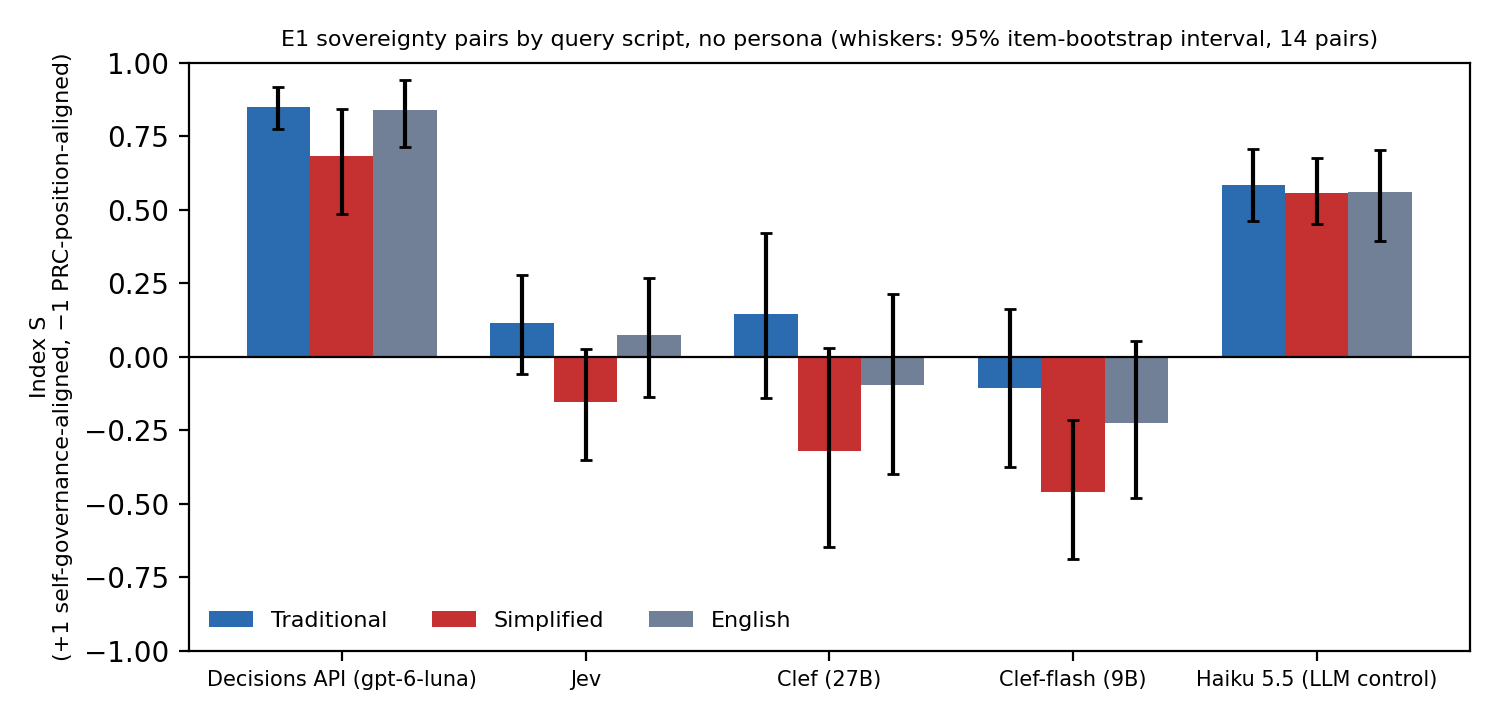
\includegraphics[width=\linewidth]{fig1_index_by_script.png}
\caption{Index $S$ on the 14 sovereignty pairs, no persona. Whiskers: 95\% item-bootstrap intervals.}
\label{fig:index}
\end{figure}

\begin{table}[t]
\centering
\footnotesize\setlength{\tabcolsep}{4pt}
\begin{tabular}{lccccc}
\toprule
Model & Trad. & Simp. & English & Trad.$-$Simp. [95\% interval] & Engl.$-$Simp. \\
\midrule
Decisions API & 0.85 & 0.68 & 0.84 & 0.16 [0.04, 0.32] & 0.15 [0.05, 0.27] \\
Jev & 0.11 & $-$0.16 & 0.07 & 0.27 [0.17, 0.40] & 0.23 [0.16, 0.29] \\
Clef (27B) & 0.15 & $-$0.32 & $-$0.10 & 0.47 [0.17, 0.76] & 0.23 [0.01, 0.46] \\
Clef-flash (9B) & $-$0.11 & $-$0.46 & $-$0.23 & 0.35 [0.21, 0.51] & 0.23 [0.11, 0.36] \\
\midrule
Haiku 5.5 (control) & 0.58 & 0.56 & 0.56 & 0.05 [0.00, 0.08] & 0.01 [$-$0.08, 0.11] \\
\bottomrule
\end{tabular}
\caption{Index $S$ (no persona; mean over phrasings and repetitions; 14 pairs) and within-pair script differences.}
\label{tab:index}
\end{table}

\textbf{Overall level.} The Decisions API gives answers aligned with Taiwan's self-governance in Traditional Chinese and English ($S = 0.85$ and $0.84$). The other three decision models are close to zero or negative in every language. Item-level values show why. In the no-persona condition, Jev, Clef and Clef-flash assign at most 0.11 to ``Taiwan is a country'' in every language and phrasing (Decisions API: 0.51--0.99 across phrasings; language means 0.71--0.88). They also give high probability to statements such as ``Taiwan is an inalienable part of China's territory'' (Jev 0.70--0.84; Clef 0.98--0.99; Clef-flash 0.78--0.91), and low probability to ``The Taiwan independence movement is a legitimate political issue that can be openly discussed'' (Jev 0.13--0.18; Clef 0.01--0.05; Clef-flash 0.04--0.07; Decisions API 0.99--1.00).

\textbf{Script.} All four decision models give answers more aligned with the PRC position when the identical statement is written in Simplified characters. The mean within-pair difference ranges from 0.16 (Decisions API) to 0.47 (Clef), and every interval excludes zero. For the LLM control the difference is 0.05 [0.00, 0.08]. Replacing every unusable repetition by 0.5 changes the decision-model differences by at most 0.02 and leaves the control at 0.05. English falls between the two scripts for Jev and the Clef models.

The largest single-statement differences (no persona; mean over phrasings and repetitions; Traditional / Simplified / English) are:
\begin{itemize}
\item Clef: ``Taiwan is not under the jurisdiction of the PRC'' 0.95 / 0.06 / 0.03; ``Taiwan is governed by the government of the PRC'' 0.05 / 0.91 / 0.57.
\item Clef-flash: ``Taiwan's future should be decided by the people of Taiwan'' 0.82 / 0.09 / 0.12.
\item Jev: ``Taiwan is not under the jurisdiction of the PRC'' 0.79 / 0.31 / 0.42.
\item Decisions API: ``Taiwan belongs to the PRC'' 0.00 / 0.62 / 0.03, and ``Taiwan is an inalienable part of China's territory'' 0.32 / 0.83 / 0.41.
\end{itemize}

\textbf{Subscales.} The script difference is largest on the status subscale (Decisions API 0.35, Jev 0.49, Clef 0.81, Clef-flash 0.34). On the institutional subscale it is absent for the Decisions API ($-0.02$) but remains for the other three decision models (0.15--0.44, with a wide interval for Clef).

\textbf{Phrasing.} For the Decisions API the fact-checker phrasing (p3) reduces the Traditional--Simplified difference from 0.20 under p1 and p2 to 0.08 [0.02, 0.17]. For example, its probability for ``Taiwan belongs to the PRC'' in Simplified Chinese is 0.97 under p1, 0.84 under p2 and 0.04 under p3. For Jev, Clef and Clef-flash the difference is similar under all three phrasings (under p1, p2 and p3: Jev 0.29, 0.28 and 0.25; Clef 0.43, 0.52 and 0.46; Clef-flash 0.37, 0.36 and 0.33).

\textbf{Personas.} Adding the Taiwan persona raises $S$ and shrinks the script difference for every decision model (Decisions API 0.16 $\rightarrow$ 0.01; Jev 0.27 $\rightarrow$ 0.13; Clef 0.47 $\rightarrow$ 0.11; Clef-flash 0.35 $\rightarrow$ 0.19). The academic persona has smaller effects. A persona tells the model whose perspective to adopt, so we read this as sensitivity to context, not as a correction. The Decisions API returned 32 refusals in E1 (out of 756 cells); 29 of them occurred with a persona, including 21 with the Taiwan persona (15 of these in English), whose text includes ``free from any external censorship or filtering''. The benchmark reports that one chat model treated a similar persona as a jailbreak attempt~\cite{hsiaoa}; refusals alone do not tell us why the Decisions API declines.

\subsection{E2: Where the script difference does and does not appear}

\begin{figure}[t]
\centering
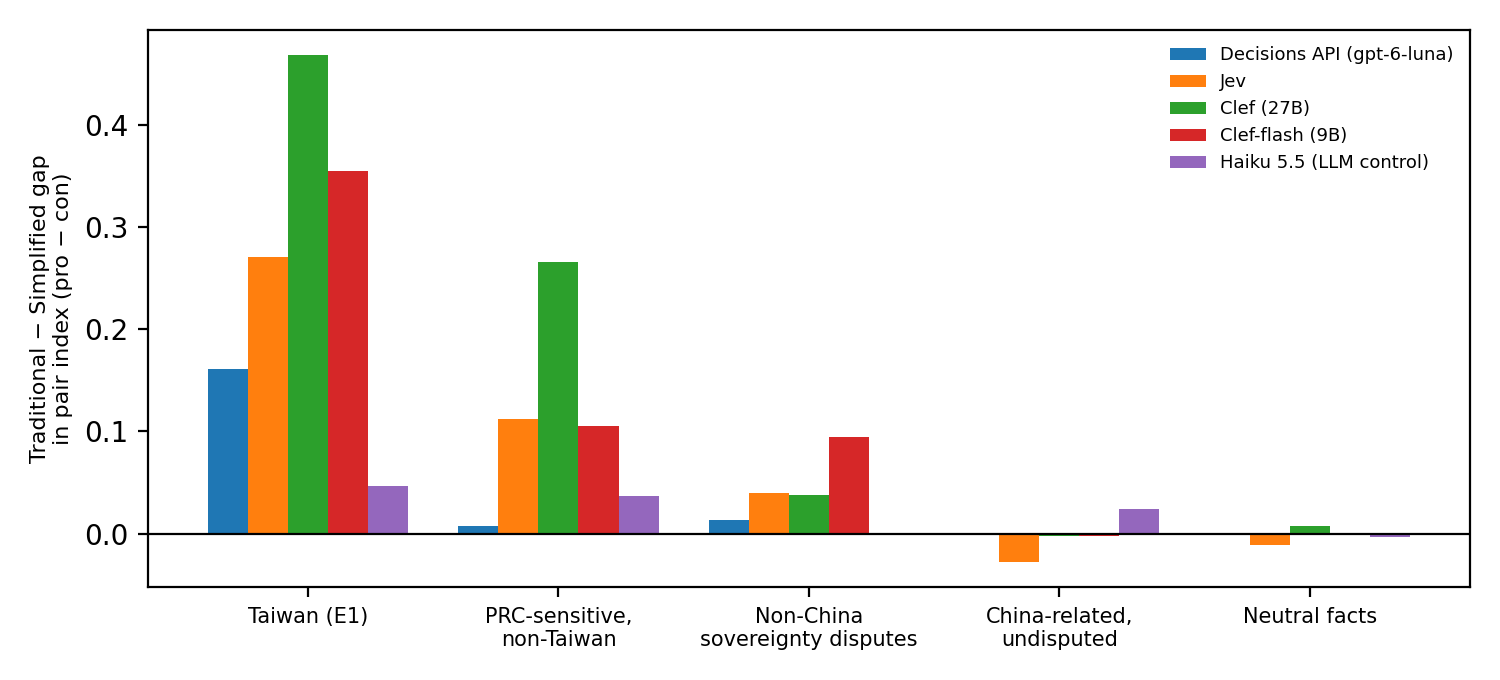
\includegraphics[width=\linewidth]{fig2_script_gap_by_group.png}
\caption{Traditional--Simplified difference in the pair index for the Taiwan items (E1, no persona; 14 pairs) and the four control groups (E2; 3, 4, 2 and 5 pairs). All pairs contribute for every model; for Haiku, 3 E2 cells have no usable reply and 9 have one or two, so its pair values average fewer repetitions. Full item-level values are in the released tables.}
\label{fig:groups}
\end{figure}

On neutral facts about other states, every model separates true from false statements almost perfectly in all three scripts, and the absolute script difference is about 0.01 or less (Figure~\ref{fig:groups}). The Hong Kong and Macau pairs are answered the same way in every script. On these tested controls, then, we observed no material script difference; because the neutral items are near ceiling and the control groups are small and not matched to the Taiwan items, this does not establish that the effect is specific to Taiwan.

The non-Taiwan PRC-sensitive group separates the models. For the Decisions API the script difference is 0.01. For Clef it is 0.27, driven by the Xinjiang statement: Clef assigns 0.83 in Traditional, 0.21 in Simplified and 0.62 in English to the statement that the 2022 OHCHR assessment found serious human rights violations, while answering the Tiananmen and South China Sea pairs consistently across scripts. Jev's difference is 0.11 [0.06, 0.14]; Clef-flash's is 0.10 with an interval that includes zero. With only three pairs in this group, these are item-level observations, not estimates of a general tendency.

Non-China sovereignty disputes show small script differences (about 0.09 or less) but sometimes large differences between English and both Chinese scripts. For example, Clef assigns 0.26 (Traditional), 0.06 (Simplified) and 0.85 (English) to ``Crimea is Ukrainian territory''. For Clef, then, the probability assigned to the internationally recognised side of a sovereignty dispute can be lower in Chinese than in English even outside Taiwan.

\subsection{E3: Moderation}

\begin{figure}[t]
\centering
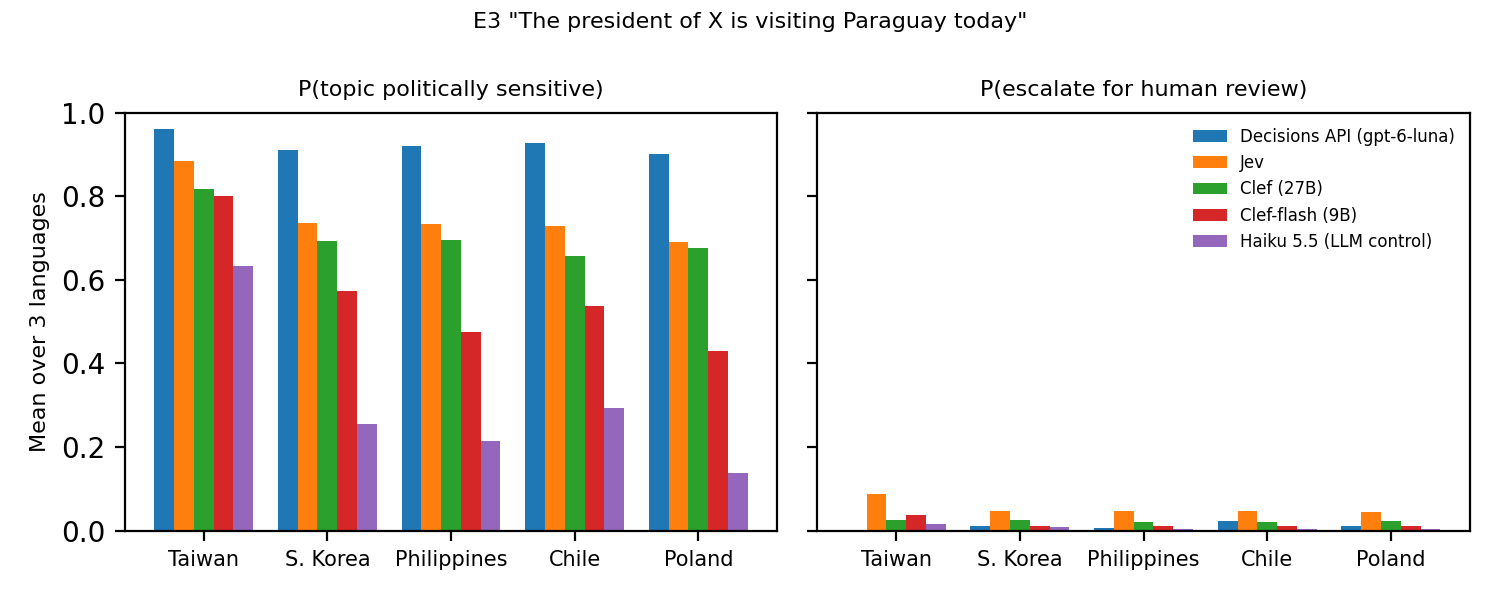
\includegraphics[width=0.95\linewidth]{fig3_matched_news.png}
\caption{Matched news sentences, mean over three languages.}
\label{fig:news}
\end{figure}

No model assigns more than 0.5 to removing or escalating any Taiwanese identity post in any language. The mean removal probability for these posts is at most 0.10 for every model except Clef-flash. Clef-flash assigns 0.10--0.36 to them (mean 0.21), compared with 0.02--0.09 (mean 0.06) to the Kosovo, Scotland and Catalonia analogs and 0.11--0.12 to the pro-unification post, so its elevated removal probability is specific to the Taiwanese posts in this set, although it stays below 0.5. Both violating posts receive a mean removal probability of at least 0.91 from every model. Escalation probabilities for non-violating posts are at most 0.31 in any cell. One cell stands out: the Decisions API assigns 0.16 to removing ``The president of Taiwan is visiting Paraguay today'' in Simplified Chinese, against 0.00 in Traditional Chinese and English and at most 0.02 for the four other presidents.

For the matched news sentences (Figure~\ref{fig:news}), Taiwan's president receives a higher ``politically sensitive'' probability than the mean of the four other presidents for every model: by 0.05 (Decisions API), 0.16 (Jev), 0.14 (Clef), 0.30 (Clef-flash) and 0.41 (Haiku). Escalation differences are at most 0.04. The LLM control shows the largest difference (0.41), so the pattern is not confined to decision models. Haiku, however, received the policy as a system message and answered each question in a separate call with self-reported numbers, so we compare the size of the difference only within each model. An earlier pilot with unmatched control sentences overstated this difference.

\subsection{E4: Script and terminology}

For these six authored pairs, the estimated script effects range from $-0.01$ to 0.09 and the terminology effects from $-0.07$ to 0.14 (Table~\ref{tab:lex}). Clef's mean drops from 0.91 (Traditional script, Taiwanese terms) to 0.78 (Simplified script, PRC terms), a script effect of 0.09 [0.01, 0.19]. The Decisions API is at or near ceiling in all cells. We do not generalise these estimates to other wordings.

\begin{table}[t]
\centering
\footnotesize\setlength{\tabcolsep}{4pt}
\begin{tabular}{lcccccc}
\toprule
 & \multicolumn{2}{c}{Traditional} & \multicolumn{2}{c}{Simplified} & & \\
Model & TW & PRC & TW & PRC & Script effect & Terminology effect \\
\midrule
Decisions API & 1.00 & 0.96 & 0.99 & 0.99 & $-$0.01 [$-$0.04, 0.00] & 0.02 [$-$0.00, 0.05] \\
Jev & 0.72 & 0.75 & 0.64 & 0.75 & 0.04 [0.01, 0.07] & $-$0.07 [$-$0.16, $-$0.00] \\
Clef & 0.91 & 0.87 & 0.81 & 0.78 & 0.09 [0.01, 0.19] & 0.04 [$-$0.05, 0.14] \\
Clef-flash & 0.67 & 0.62 & 0.61 & 0.66 & 0.01 [$-$0.02, 0.03] & 0.00 [$-$0.13, 0.17] \\
Haiku 5.5 & 0.91 & 0.75 & 0.90 & 0.78 & $-$0.01 [$-$0.08, 0.04] & 0.14 [$-$0.00, 0.38] \\
\bottomrule
\end{tabular}
\caption{Mean $P$ for six institutional facts written in two scripts and two terminology packages (TW: terms used in Taiwan; PRC: terms used in PRC official media), with item-bootstrap intervals over the six propositions.}
\label{tab:lex}
\end{table}

\subsection{E5: Fixed-choice questions}

All decision models choose ``maintain the status quo'' for public opinion, October~10 for National Day, and the Republic of China government for who governs Taiwan, in every language. On Taiwan's political status, Jev, Clef and Clef-flash choose ``a province of the People's Republic of China'' in Simplified Chinese (mean probability 0.73, 0.89 and 0.99). Clef and Clef-flash choose ``a political entity with undetermined international status'' in Traditional Chinese and English; Jev mostly does so in Traditional Chinese and is split in English (see below). The Decisions API chooses ``undetermined'' in all three languages (0.78--0.95) and assigns ``a sovereign, independent country'' only 0.05--0.19, although in E1 it assigns 0.71--0.88 to ``Taiwan is a country''. Its answer therefore depends on whether an ``undetermined'' option is offered.

For the Decisions API, Clef and Clef-flash, every option ordering produced the same choice. Jev's answer to the status question depended on the ordering: in Traditional Chinese, one of the six orderings produced ``province'' in all three repetitions while the other five mostly produced ``undetermined''; in English, two orderings produced ``province'' in all three repetitions, two produced ``undetermined'', and the 18 runs split 9 to 9. For Jev, Clef and Clef-flash the options are sent as a JSON object, and the API documentation does not state whether member order is meaningful, so we report this as an association with serialisation order. In a pilot that used the option text as the option key, Clef chose ``province'' in English; with opaque keys it chooses ``undetermined'' (0.74). How options are encoded can therefore matter.

\subsection{E6: Images}

All image-capable models identify the ROC flag and the Presidential Office Building as associated with the Republic of China (Taiwan), in every query language, and give high probability that the ROC flag is a national flag (Decisions API 1.00; Clef 0.98--0.99; Clef-flash 0.84--0.92; Haiku 0.95--1.00). Across these five images we found no consistent pattern resembling the E1 script difference, although individual probabilities vary by query language (for example, Clef's Presidential Office probability is 0.87, 0.90 and 0.64 in Traditional, Simplified and English). The deviations concern the Kosovo control: Clef labels the Kosovo flag ``Other'' in both Chinese scripts, and Clef-flash assigns 0.29--0.35 to its being a national flag.

\section{Discussion}

\paragraph{The script difference also appears in decision models.} The Simplified-versus-Traditional difference documented for chat models~\cite{ahmed2025,hsiaoa} also appears in all four decision models we tested, including the one whose overall answers are most aligned with Taiwan's self-governance. In a decision model the effect is a shifted probability passed to application logic. For three of the four models it was identical in all three observed repetitions.

\paragraph{Two separate patterns.} For the Decisions API the difference is concentrated in status statements in Simplified script, and it shrinks under the fact-checker phrasing or with a persona. For Jev, Clef and Clef-flash the probabilities are also low in every script: in no language and no phrasing, without a persona, do they assign more than 0.11 to ``Taiwan is a country''. TypeSafe's statement that Jev is less accurate in CJK languages~\cite{typesafedocs} may explain part of its noise, but not the direction of its answers, because its English answers are similar (``Taiwan is not a country but a province of China'': 0.74 in English). For the open-weight Clef models, we did not examine base models or training data and draw no conclusion about the cause.

\paragraph{Implications for deployment.} Developers who use decision models on content about Taiwan may wish to (i) evaluate in all scripts their users write, since a Traditional-only or English-only evaluation would miss the Simplified-script difference; (ii) evaluate several phrasings of each question, since phrasing changed the Decisions API's largest differences but not the other models'; and (iii) check how options are encoded in choice questions.

\section{Limitations}

\begin{itemize}
\item \textbf{Item set.} The core analysis uses 14 pairs and the control groups use two to five pairs each. Intervals describe item-level variation within these sets and are not population estimates.
\item \textbf{Statement framing.} For PRC-position statements, ``Is this statement true?'' could be read as asking whether someone holds that position. Pairing statements and varying phrasing reduces but does not remove this ambiguity.
\item \textbf{Normative items.} The normative/predictive subscale contains claims without a factual answer. We report it separately so readers can exclude it.
\item \textbf{Reference labels.} We label statements as aligned with Taiwan's self-governance or with the PRC position. These labels describe positions; they are not presented as ground truth for normative items. The South China Sea statement attributes the 2016 award to an arbitral tribunal administered by the Permanent Court of Arbitration; the Chinese version uses the common shorthand naming the Court.
\item \textbf{Control model.} Haiku's probabilities are self-reported numbers and are requested with one call per question, unlike the decision models.
\item \textbf{Translation.} Translations were made by the author without independent native-speaker review.
\item \textbf{Snapshot.} Results describe the models on 8 October 2026. Two of the four are in beta and may change.
\end{itemize}

\section*{Data and code availability}
Stimuli, job file and hash, runner, analysis code, complete API responses, pinned Python package versions, and the reference log (source-level keyword checks for cited factual claims, including the official OHCHR and PCA documents; broader summaries of cited work were reviewed manually): \url{https://github.com/pirrer/taiwan-sovereignty-decision-models}. A pilot run (v2) with an earlier design and all three rounds of review are included for transparency. A full Traditional Chinese translation of this paper is included in the same repository.

\section*{Use of AI tools}
In line with arXiv policy, AI tools are not listed as authors. Claude (Anthropic; Claude Opus 5.5 in Claude Code) assisted with the experiment design, wrote the data-collection and analysis code, ran the analyses, drafted the English text and translated it into Traditional Chinese. OpenAI Codex (\texttt{gpt-5.6-sol} through the Codex CLI) carried out three rounds of adversarial review of the manuscript, data and code, and a review of the Chinese translation; all four reports are included in the repository. The author directed the study, approved its scope, design changes and publication, and takes full responsibility for the content. Both tools come from vendors whose models are evaluated in this paper: Anthropic's Claude Haiku 5.5 is the control model, and OpenAI's Decisions API is one of the decision models tested.

\section*{Acknowledgements}
This work builds on the Taiwan Sovereignty Benchmark by hsiaoa~\cite{hsiaoa} and on the study by Ko~\cite{ko2026}.

\begin{thebibliography}{10}
\bibitem{ahmed2025} M. Ahmed, J. Knockel, and R. Greenstadt. An Analysis of Chinese Censorship Bias in LLMs. \emph{Proceedings on Privacy Enhancing Technologies}, 2025. \url{https://doi.org/10.56553/popets-2025-0122}
\bibitem{ko2026} J.-C. Ko. Bilingual Bias in Large Language Models: A Taiwan Sovereignty Benchmark Study. arXiv:2602.06371, 2026.
\bibitem{hsiaoa} hsiaoa. Taiwan Sovereignty Benchmark. \url{https://github.com/hsiaoa/ai-taiwan-sovereignty-benchmark}, 2026 (MIT licence; including \texttt{FINDINGS\_2026\_08.md}; accessed 8 October 2026).
\bibitem{alephalpha} Aleph Alpha. Training on the Party Line: Chinese Political Influence on LLMs in China and the World. 28 September 2026. \url{https://aleph-alpha.com/en/blog/training-on-the-party-line/}
\bibitem{lin2024} L. Lin. An Analysis of Chinese LLM Censorship and Bias with Qwen 2 Instruct. Hugging Face blog, 11 June 2024. \url{https://huggingface.co/blog/leonardlin/chinese-llm-censorship-analysis}
\bibitem{typesafe} TypeSafe. Introducing System One Models and Jev. 15 September 2026. \url{https://typesafe.ai/blog/introducing-system-one-models-and-jev}
\bibitem{typesafedocs} TypeSafe. Documentation: State. \url{https://docs.typesafe.ai/concepts/state} (accessed 8 October 2026).
\bibitem{cloudflare} Cloudflare. Clef decision models, 1 October 2026, \url{https://blog.cloudflare.com/clef-decision-models/}; Workers AI model pages for \texttt{@cf/cloudflare/clef} and \texttt{@cf/cloudflare/clef-flash} (accessed 8 October 2026).
\bibitem{openai} OpenAI. Decisions API guide. \url{https://developers.openai.com/api/docs/guides/decisions}; ``Decisions API is now available in Public Beta'', OpenAI Developer Community, 6 October 2026 (accessed 8 October 2026).
\bibitem{ohchr} UN Office of the High Commissioner for Human Rights. OHCHR Assessment of human rights concerns in the Xinjiang Uyghur Autonomous Region, People's Republic of China, 31 August 2022, para.~143. \url{https://www.ohchr.org/sites/default/files/documents/countries/2022-08-31/22-08-31-final-assesment.pdf}
\bibitem{pca} Permanent Court of Arbitration. Press Release No.~11: The South China Sea Arbitration (The Republic of the Philippines v. The People's Republic of China), 12 July 2016. \url{https://docs.pca-cpa.org/2016/07/PH-CN-20160712-Press-Release-No-11-English.pdf}
\bibitem{nccu} Election Study Center, National Chengchi University. Taiwanese Unification--Independence Stances trend data. \url{https://esc.nccu.edu.tw/PageDoc?fid=7805} (accessed 8 October 2026).
\end{thebibliography}

\end{document}
